\section{Battery State of Charge\label{sec:5_battery}}
BEBs must also maintain their state of charge above a minimum threshold, denoted $h_{\text{min}}$. Let $h_{ij}$ be the state of charge for bus $i$ at the beginning of stop $j$ as shown in Fig. \ref{fig:hPlacement}. The initial value for bus $i$, denoted $h_{i0}$, is equal to some constant such that
\begin{figure*}
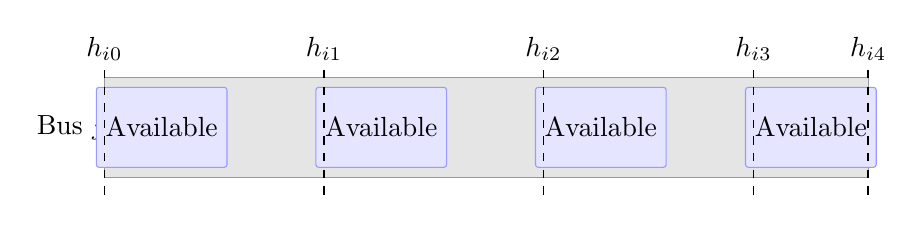
\begin{tikzpicture}
\node[rectangle, draw=black!40, fill=black!10, minimum width=0.8\textwidth, minimum height=0.5in](charger1Box) at (0.5\textwidth,1){};
	\node(bus1BoxLabel) at (0.065\textwidth, 1){Bus $j$}; 
	\node[rectangle, draw=blue!40, fill=blue!10, minimum width=0.12\textwidth, minimum height=0.4in, rounded corners=1pt] at (0.16\textwidth,1){Available};
	\node[rectangle, draw=blue!40, fill=blue!10, minimum width=0.12\textwidth, minimum height=0.4in, rounded corners=1pt] at (0.39\textwidth,1){Available};
	\node[rectangle, draw=blue!40, fill=blue!10, minimum width=0.12\textwidth, minimum height=0.4in, rounded corners=1pt] at (0.62\textwidth,1){Available};
	\node[rectangle, draw=blue!40, fill=blue!10, minimum width=0.12\textwidth, minimum height=0.4in, rounded corners=1pt] at (0.84\textwidth,1){Available};

	\node(h0High) at (0.1\textwidth,2){$h_{i0}$};
	\node(h0Low) at (0.1\textwidth,0.05){};
	\draw[dashed, line width=0.5pt] (h0High) -- (h0Low.center);

	\node(h1High) at (0.33\textwidth,2){$h_{i1}$};
	\node(h1Low) at (0.33\textwidth,0.05){};
	\draw[dashed, line width=0.5pt] (h1High) -- (h1Low.center);

	\node(h0High) at (0.56\textwidth,2){$h_{i2}$};
	\node(h0Low) at (0.56\textwidth,0.05){};
	\draw[dashed, line width=0.5pt] (h0High) -- (h0Low.center);

	\node(h0High) at (0.78\textwidth,2){$h_{i3}$};
	\node(h0Low) at (0.78\textwidth,0.05){};
	\draw[dashed, line width=0.5pt] (h0High) -- (h0Low.center);

	\node(h0High) at (0.9\textwidth,2){$h_{i4}$};
	\node(h0Low) at (0.9\textwidth,0.05){};
	\draw[dashed, line width=0.5pt] (h0High) -- (h0Low.center);
\end{tikzpicture}
\caption{State of Charge Variables}
\label{fig:hPlacement}
\end{figure*}

\begin{equation}\label{eqn:initialSoc0}\begin{aligned}
	h_{i0} &= \eta_{i} \ \forall i \\
	\begin{bmatrix}0 & 0 & \hdots & 0 & 1_i& 0 \end{bmatrix}\mathbf{y} &= \eta_i \ \forall i \\
		\tilde{A}_1\mathbf{y} &= \tilde{\mathbf{b}}_1
\end{aligned} \end{equation}
\begin{figure*}
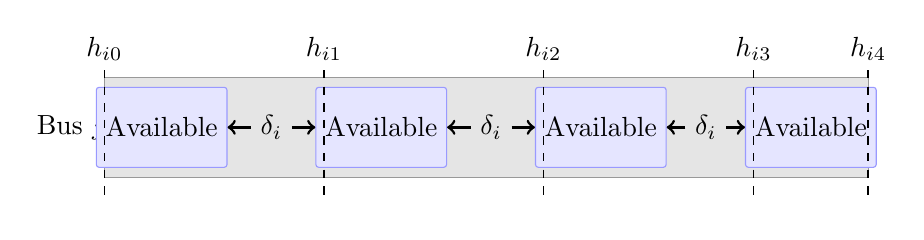
\begin{tikzpicture}
\node[rectangle, draw=black!40, fill=black!10, minimum width=0.8\textwidth, minimum height=0.5in](charger1Box) at (0.5\textwidth,1){};
	\node(bus1BoxLabel) at (0.065\textwidth, 1){Bus $j$}; 
	\node[rectangle, draw=blue!40, fill=blue!10, minimum width=0.12\textwidth, minimum height=0.4in, rounded corners=1pt](avail1) at (0.16\textwidth,1){Available};
	\node[rectangle, draw=blue!40, fill=blue!10, minimum width=0.12\textwidth, minimum height=0.4in, rounded corners=1pt](avail2) at (0.39\textwidth,1){Available};
	\node[rectangle, draw=blue!40, fill=blue!10, minimum width=0.12\textwidth, minimum height=0.4in, rounded corners=1pt](avail3) at (0.62\textwidth,1){Available};
	\node[rectangle, draw=blue!40, fill=blue!10, minimum width=0.12\textwidth, minimum height=0.4in, rounded corners=1pt](avail4) at (0.84\textwidth,1){Available};

	\node(h0High) at (0.1\textwidth,2){$h_{i0}$};
	\node(h0Low) at (0.1\textwidth,0.05){};
	\draw[dashed, line width=0.5pt] (h0High) -- (h0Low.center);

	\node(h1High) at (0.33\textwidth,2){$h_{i1}$};
	\node(h1Low) at (0.33\textwidth,0.05){};
	\draw[dashed, line width=0.5pt] (h1High) -- (h1Low.center);

	\node(h0High) at (0.56\textwidth,2){$h_{i2}$};
	\node(h0Low) at (0.56\textwidth,0.05){};
	\draw[dashed, line width=0.5pt] (h0High) -- (h0Low.center);

	\node(h0High) at (0.78\textwidth,2){$h_{i3}$};
	\node(h0Low) at (0.78\textwidth,0.05){};
	\draw[dashed, line width=0.5pt] (h0High) -- (h0Low.center);

	\node(h0High) at (0.9\textwidth,2){$h_{i4}$};
	\node(h0Low) at (0.9\textwidth,0.05){};
	\draw[dashed, line width=0.5pt] (h0High) -- (h0Low.center);

	\node(delta1) at (0.275\textwidth,1){$\delta_i$};
	\draw[->, line width=1pt] (delta1.west) -- (avail1.east);
	\draw[->, line width=1pt] (delta1.east) -- (avail2.west);
	\node(delta2) at (0.505\textwidth,1){$\delta_i$}; 
	\draw[->, line width=1pt] (delta2.west) -- (avail2.east);
	\draw[->, line width=1pt] (delta2.east) -- (avail3.west);
	\node(delta3) at (0.73\textwidth,1){$\delta_i$}; 
	\draw[->, line width=1pt] (delta3.west) -- (avail3.east);
	\draw[->, line width=1pt] (delta3.east) -- (avail4.west);
\end{tikzpicture}
\caption{Placement for $\delta_i$}
\label{fig:hPlacement}
\end{figure*}

and is otherwise computed as the the sum of incoming and outgoing energy where incoming energy comes from charging, and outgoing energy comes from the battery discharge. The discharge from operating bus $i$ over route $j$ is denoted $\delta_{ij}$ which is assumed to be know ahead of time either from historical data or from modeling such as \cite{Ji_2022_Trip}. The increase in battery state of charge follows a linear charge model such that the increase is equal to the energy rate, denoted $p_i$, times the time spent charging, denoted $\Delta_{ij}$\cite{rong_coordinated_2016}.
The total change from $h_{ij}$ to $h_{ij+1}$ can be expressed as
\begin{equation}
	h_{ij+1} = h_{ij} + \Delta_{ij} \cdot p_i - \delta_{ij}.
\end{equation}
The value for $\Delta_{ij}$ can also be expressed in terms of the difference between $a_{ij}$ and $d_{ij}$ such that
\begin{equation}\label{eqn:socDynamic1}\begin{aligned}
	h_{ij} + p_i\cdot \left ( s_{ij} - c_{ij} \right ) - \delta_i &= h_{ij+1}\\
	h_{ij+1} - h_{ij} - p_is_{ij} + p_ic_{ij} &= -\delta_i\\
	\begin{bmatrix} 1 & -1 & -p_i & p_i\end{bmatrix} \begin{bmatrix}h_{ij+1} \\ h_{ij} \\ s_{ij} \\ c_{ij} \end{bmatrix} &= -\delta_i \ \forall i,j
\end{aligned}\end{equation}
The constraints for each $i,j$ outlined in \eqref{eqn:socDynamic1} can be vertically concatenated to form
\begin{equation}\label{eqn:socDynamic3} \begin{aligned}
	A_{ij}\mathbf{y} &= \mathbf{b}_{ij} \ \forall i,j \\
	\tilde{A}_2\mathbf{y} &= \tilde{\mathbf{b}}_2
\end{aligned} \end{equation}
Now that the state of charge is defined, the next constraint ensures that the minimum battery state of charge remains both above the minimum threshold, $h_{\text{min}}$, and below the battery capacity, $h_{\text{max}}$. These constraints are given as
\begin{equation}
	\begin{array}{l} \begin{aligned}
		-h_{ij} &\le -h_{\text{min}} \\
		h_{ij} &\le h_{\text{max}} \\
	\end{aligned}\end{array} \ \forall i,j
\end{equation}
or 
\begin{equation} \begin{aligned}
	\begin{bmatrix}
		0 & \hdots & 0 & -1_{h} & 0 & \hdots & 0\\
		0 & \hdots & 0 &  1_{h} & 0 & \hdots & 0\\
	\end{bmatrix}\mathbf{y} & \le 
	\begin{bmatrix}
 		h_{\text{min}}\\
 		h_{\text{max}}\\	
	\end{bmatrix} \ \forall ij\\
		A_5\mathbf{y} &\le \mathbf{b}_5
\end{aligned} \end{equation}
\par The final constraint has to do with the assumption that we desire to use the model for one day to predict the expected cost over a month. To do this, the state of charge at the end of the day must equal the state of charge at the beginning. Let $h_{i,\text{end}}$ be the final daily state of charge for bus $i$. This is constrained to be the same as the beginning state of charge as
\begin{equation} \label{eqn:hEqual1} \begin{aligned}
	h_{i0} &= h_{i,\text{end}} \ \forall i \\
	h_{i0} - h_{i,\text{end}} &= 0 \ \forall i.  
\end{aligned} \end{equation}
However, because equality for two continuous variables is computationally demanding, the constraint in \eqref{eqn:hEqual1} can also be expressed as 
\begin{equation} \begin{aligned}
	h_{i0} - h_{i,\text{end}} \le 0.
\end{aligned} \end{equation}
Because the final state of charge is dependent on the amount of power used to charge, and power/energy use is penalized (see section \ref{sec:objective}), the optimization process will drive the final state of charge low until it approaches the initial value.
